\chapter{Delotoki v Orangeu}
\label{ch:workflows}

\newthought{Delotoki v Orangeu} so sestavljeni iz komponent, ki berejo, procesirajo in prikazujejo podatke. Te komponente imenujemo gradniki oz gradniki. Na desni je prazen prostor, t.i. platno. Nanj polagamo gradnike. Gradniki v Orangeu komunicirajo preko komunikacijskih kanalov. Izhod iz enega gradnika je uporabljen kot vhod za drug gradnik.

\begin{figure*}[h]
  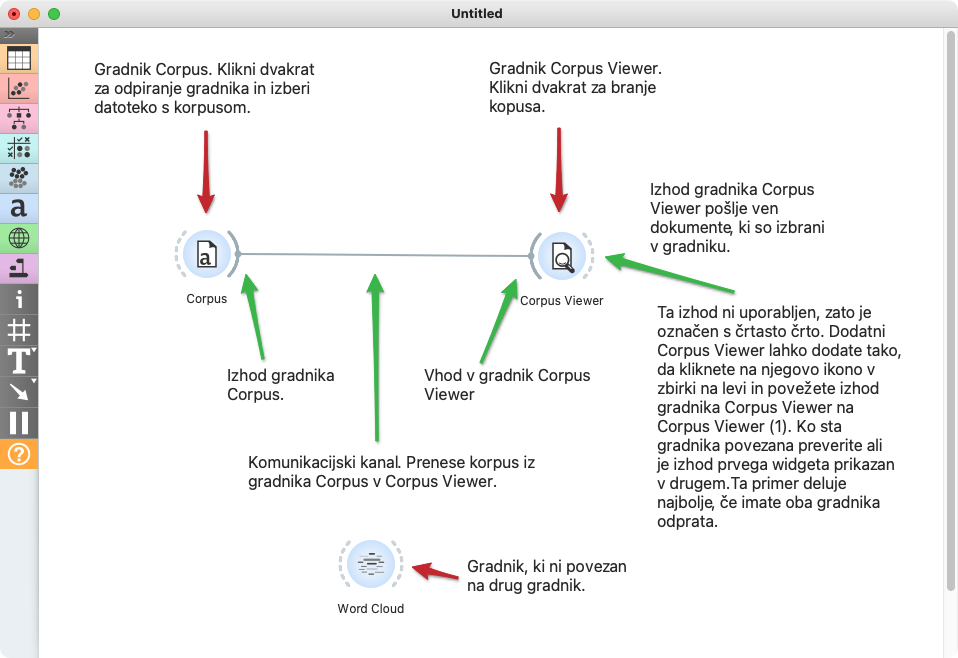
\includegraphics[width=\linewidth]{workflow-fig1.png}%
  \caption{Slika zgoraj kaže preprost delotok z dvema povezanima gradnikoma in enim gradnikom brez povezav. Izhodi gradnika so na desni strani, vhodi pa na levi.}
  \label{fig:workflow-fig1}
\end{figure*}

Delotoke sestavljamo tako, da polagamo gradnike na platno in jih povezujemo. Povezavo ustvarimo tako, da potegnemo črto od izhodnega v vhodni gradnik. Izhodi gradnika so na desni, vhodi pa na levi strani. V zgornjem delotoku gradnik \textit{Corpus} pošilja podatke v gradnik \textit{Corpus Viewer}.

\newpage

Pričnite z gradnjo delotoka, ki vsebuje gradnik \textit{Corpus}, dva gradnika \textit{Corpus Viewer} in gradnika \textit{Word Cloud}:

\begin{figure}[h]
  \centering
  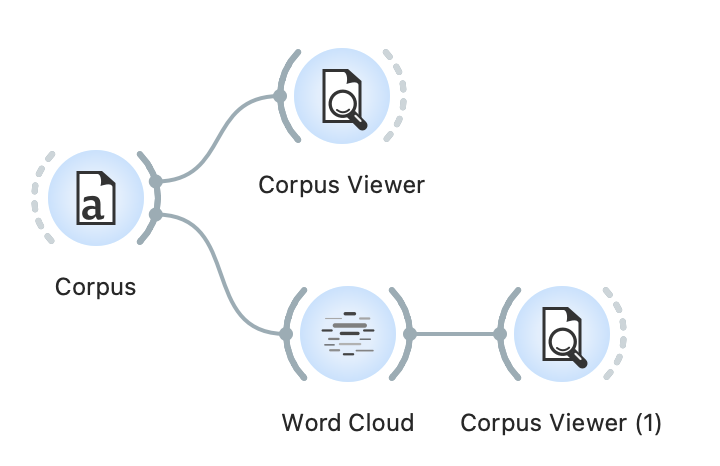
\includegraphics[width=0.9\linewidth]{workflow-ex.png}%
  \caption{Delotok z gradnikom Corpus bere podatke iz računalnika in jih pošlje v gradnika Corpus Viewer in Word Cloud.  Corpus Viewer prikaže besedila v iskalniku, Word Cloud pa izriše najpogostejše besede. Dokumenti, ki vsebujejo izbrano besedo iz gradnika Word Cloud, so prikazani v gradniku Corpus Viewer (1).}
  \label{fig:workflow-fig2}
\end{figure}

Gradnik \textit{Corpus} bere podatke iz lokalnega diska. Odprite Corpus tako, da dvakrat kliknete na ikono. Dodatek Text že vsebuje nekaj prednaloženih korpusov. Iz teh (“Browse”) izberite \textit{Grimms-tales-selected.tab}, korpus z izbranimi Grimmovimi pravljicami. 

\begin{figure}[h]
  \centering
  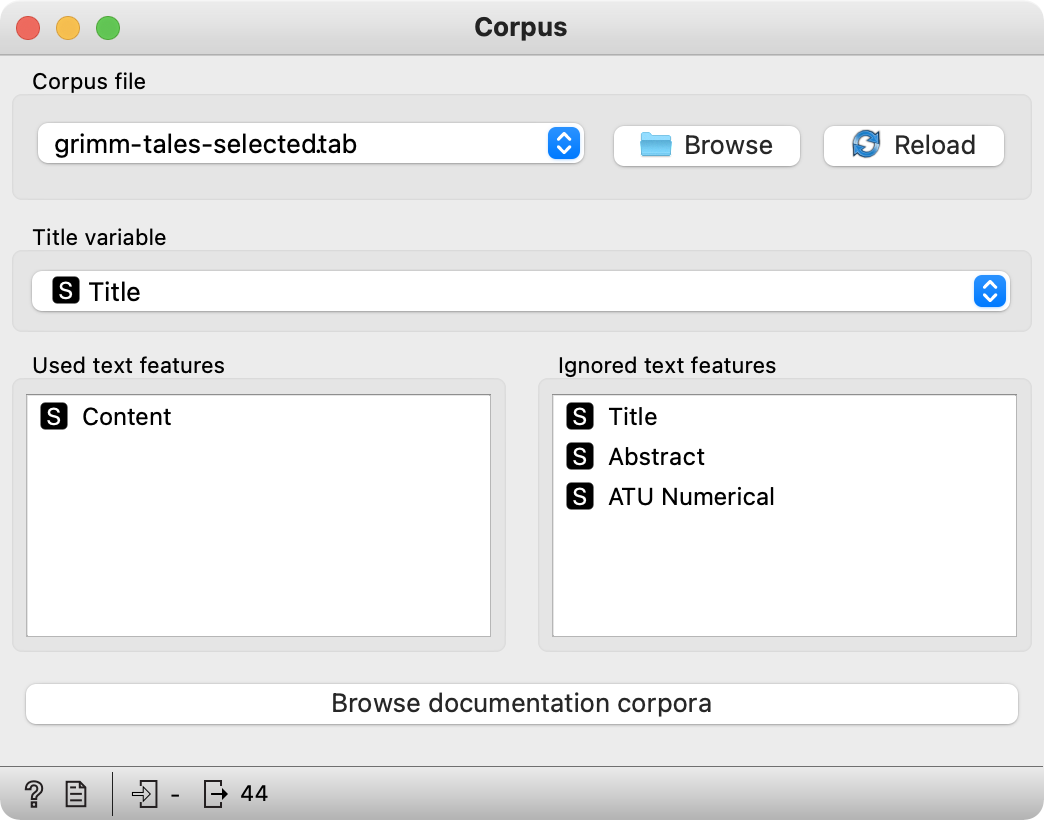
\includegraphics[width=\linewidth]{corpus.png}%
  \caption{Orangevi delotoki se pogosto pričnejo z gradnikoma File ali Corpus. Korpus Grimmovih pravljic vsebuje 44 dokumentov.  Polje “Used text features”na levi pove, katere stolpce bomo smatrali kot del besedila, medtem ko polje na desni vsebuje dodatne informacije (naslov, povzetek, itd.).}
  \label{fig:workflow-fig3}
\end{figure}

Odprite \textit{Word Cloud}. Word Cloud (oblak besed) prikaže pogostost besed v dokumentih, kjer so pogosteješe besede prikazane sorazmerno večje. Izberite besedo v oblaku in jo pošiljte v Corpus Viewer (1). Sedaj lahko pregledate samo dokumente, ki vsebujejo izbrano besedo.

\newpage

\begin{figure}[h]
  \centering
  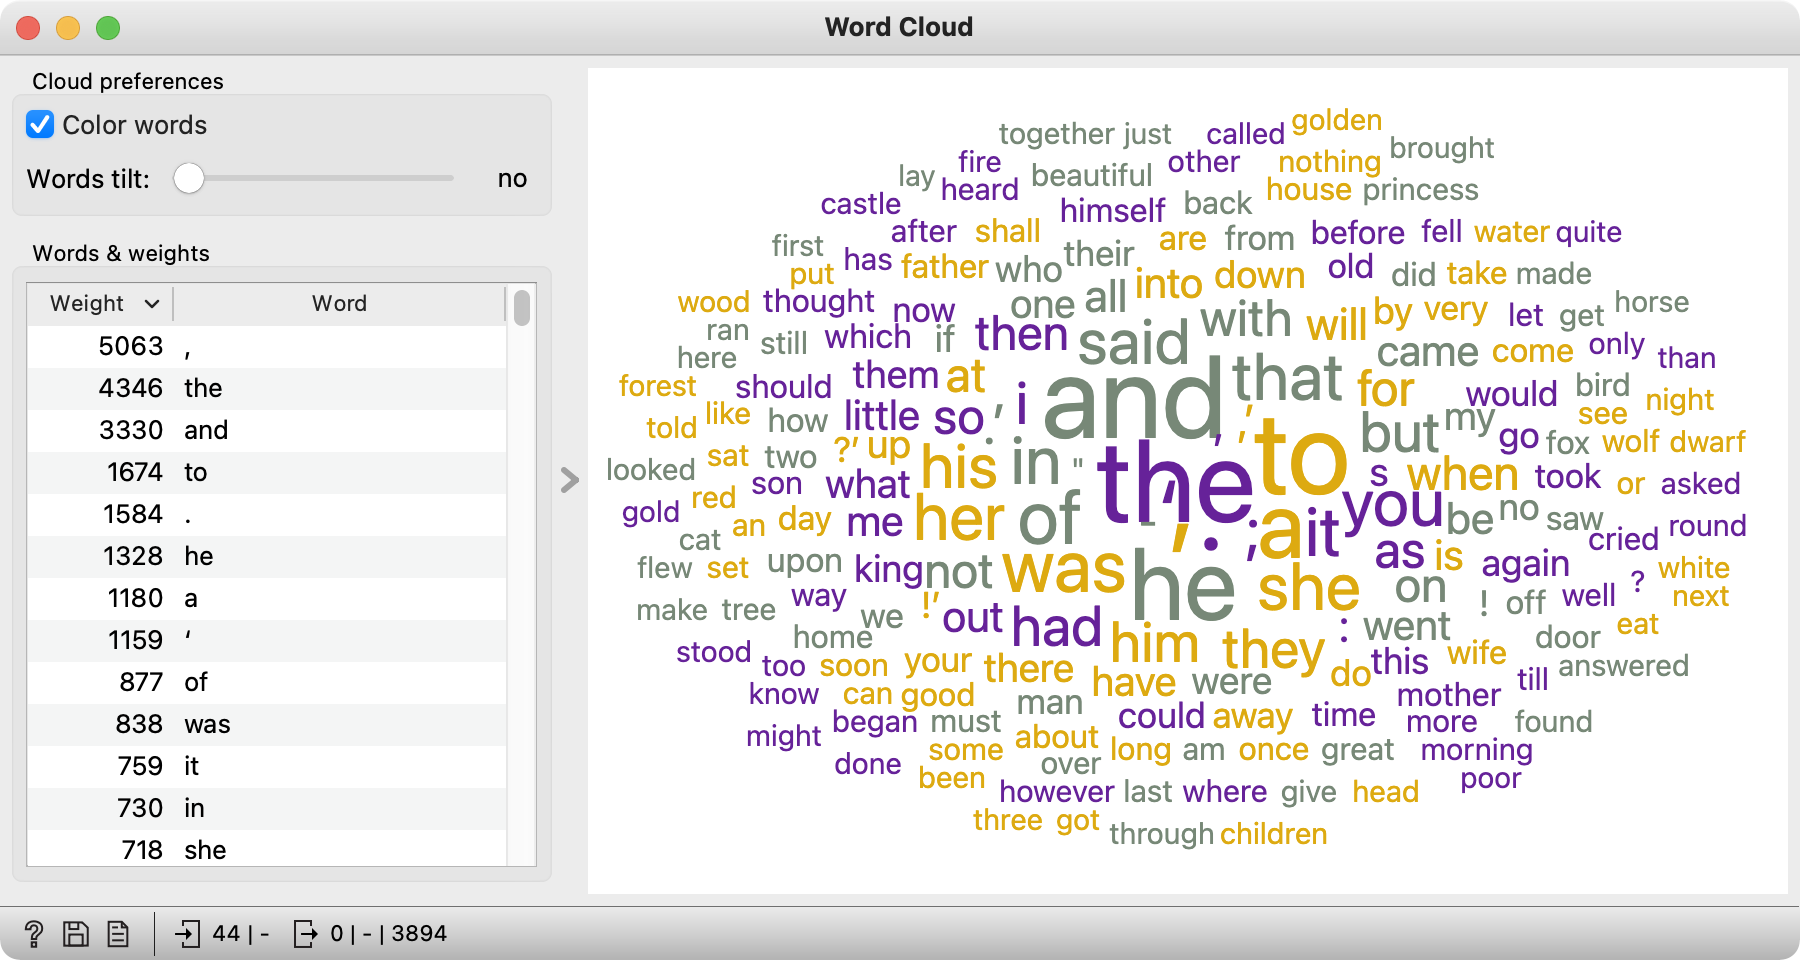
\includegraphics[width=\linewidth]{word-cloud.png}
\end{figure}

Počakajmo malo! Ta oblak besed je živa groza! Vidimo lahko celo kopico semantičnih smeti.  Ali obstaja kakšen način, da to nekako uredimo?

Seveda! Odstraniti moramo vse delčke, ki ne vsebujejo nikakršne informacije, točneje ločila in odvečne besede (členke, pomožne glagole, veznike).